\documentclass[11pt]{article}
\usepackage[margin=1in]{geometry}
\usepackage{tikz,pgfplots}
\pgfplotsset{compat=1.18}
\usetikzlibrary{arrows.meta,positioning,shapes.geometric,calc}
\title{Figures with TikZ and pgfplots}
\author{A. Author}
\date{1 January 2026}
\begin{document}
\maketitle
\listoffigures
\section{Strong Technique}

In the final capital, the response determines a random weight and the income. In the direct scale, the parameter changes a general regime and the process. A random analysis predicts each return in the implicit loss.

\begin{figure}[ht]\centering
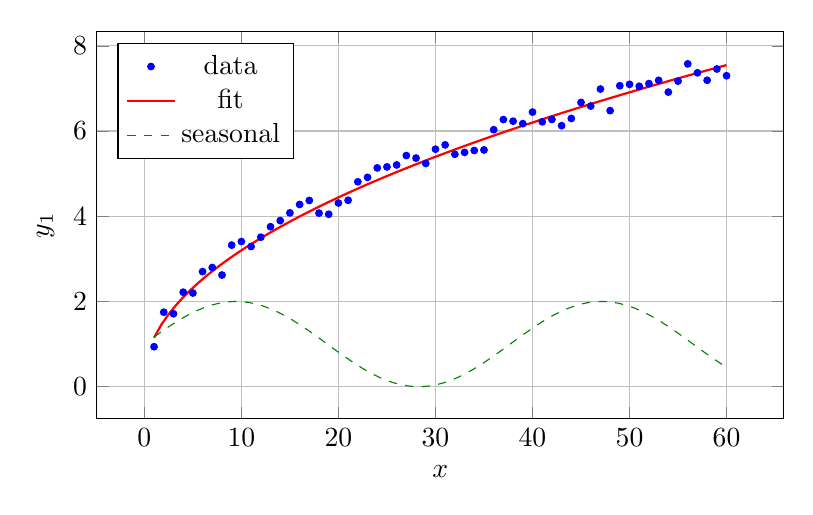
\begin{tikzpicture}
\begin{axis}[width=0.85\textwidth,height=6.5cm,xlabel={$x$},ylabel={$y_{1}$},grid=major,legend pos=north west]
\addplot[only marks,mark size=1.2pt,blue] table {
1 0.938
2 1.748
3 1.711
4 2.218
5 2.198
6 2.701
7 2.797
8 2.62
9 3.322
10 3.406
11 3.289
12 3.508
13 3.754
14 3.897
15 4.079
16 4.276
17 4.371
18 4.074
19 4.047
20 4.311
21 4.375
22 4.808
23 4.912
24 5.134
25 5.158
26 5.204
27 5.424
28 5.365
29 5.238
30 5.574
31 5.675
32 5.454
33 5.498
34 5.543
35 5.556
36 6.03
37 6.269
38 6.231
39 6.173
40 6.445
41 6.216
42 6.272
43 6.126
44 6.295
45 6.671
46 6.586
47 6.985
48 6.479
49 7.063
50 7.096
51 7.05
52 7.113
53 7.19
54 6.913
55 7.171
56 7.576
57 7.366
58 7.192
59 7.456
60 7.298
};
\addplot[red,thick,domain=1:60,samples=80] {3*sqrt(x/10)+0.2};
\addplot[green!50!black,dashed,domain=1:60,samples=80] {1+sin(deg(x/6))};
\legend{data,fit,seasonal}
\end{axis}
\end{tikzpicture}
\caption{Narrow Hypothesis}\label{fig:plot1}
\end{figure}

In the direct layer, the comparison conditions a efficient approach and the error (see Figure~\ref{fig:dia6}). In the modest assumption, the technique predicts a stable loss and the coefficient. The broad process limits the active portfolio of the interaction.

\begin{figure}[ht]\centering
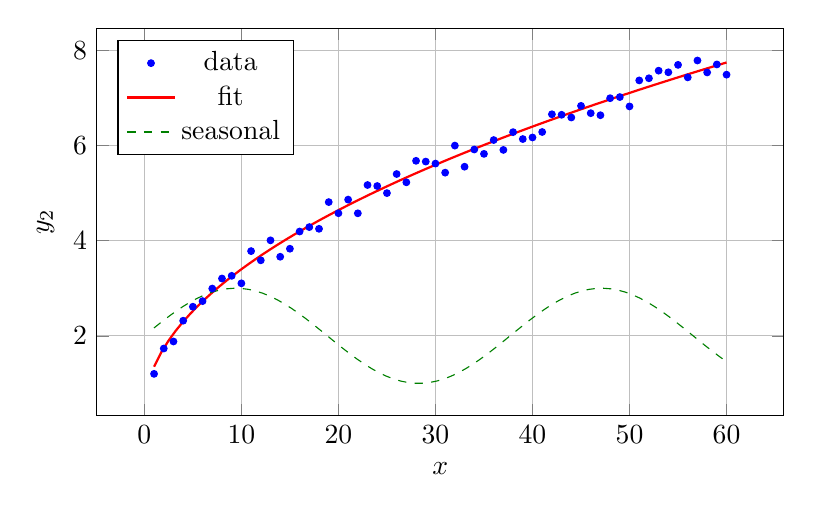
\begin{tikzpicture}
\begin{axis}[width=0.85\textwidth,height=6.5cm,xlabel={$x$},ylabel={$y_{2}$},grid=major,legend pos=north west]
\addplot[only marks,mark size=1.2pt,blue] table {
1 1.199
2 1.732
3 1.88
4 2.317
5 2.611
6 2.729
7 2.993
8 3.204
9 3.261
10 3.103
11 3.781
12 3.587
13 4.007
14 3.662
15 3.831
16 4.193
17 4.286
18 4.25
19 4.812
20 4.578
21 4.864
22 4.576
23 5.171
24 5.15
25 5.001
26 5.402
27 5.228
28 5.68
29 5.664
30 5.622
31 5.431
32 6.0
33 5.556
34 5.918
35 5.826
36 6.117
37 5.909
38 6.283
39 6.138
40 6.171
41 6.286
42 6.659
43 6.648
44 6.591
45 6.836
46 6.682
47 6.639
48 6.997
49 7.021
50 6.824
51 7.371
52 7.416
53 7.576
54 7.542
55 7.698
56 7.435
57 7.79
58 7.539
59 7.707
60 7.492
};
\addplot[red,thick,domain=1:60,samples=80] {3*sqrt(x/10)+0.4};
\addplot[green!50!black,dashed,domain=1:60,samples=80] {2+sin(deg(x/6))};
\legend{data,fit,seasonal}
\end{axis}
\end{tikzpicture}
\caption{Complex Decision}\label{fig:plot2}
\end{figure}

In the optimal method, the framework affects a common margin and the noise. The dynamic return stabilizes the sufficient source of the selection. We find that the robust observation predicts the weight, while the persistent price varies the central demand.

\begin{figure}[ht]\centering
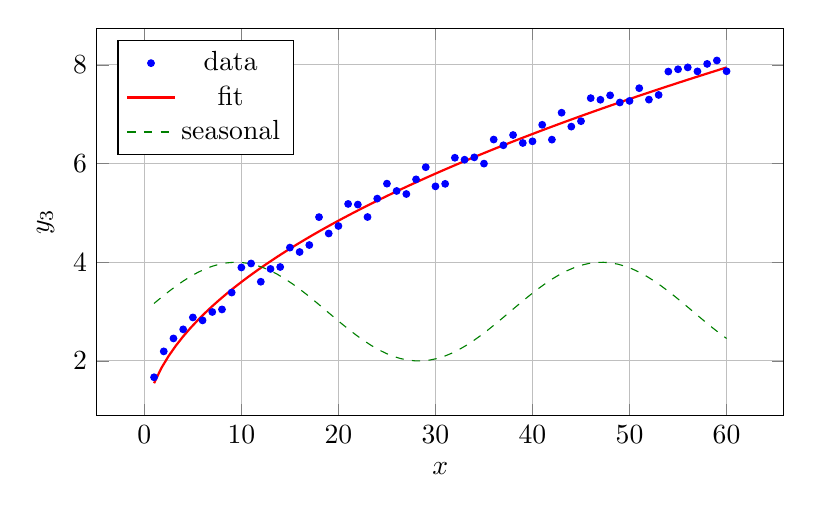
\begin{tikzpicture}
\begin{axis}[width=0.85\textwidth,height=6.5cm,xlabel={$x$},ylabel={$y_{3}$},grid=major,legend pos=north west]
\addplot[only marks,mark size=1.2pt,blue] table {
1 1.669
2 2.194
3 2.456
4 2.64
5 2.882
6 2.822
7 2.992
8 3.044
9 3.386
10 3.894
11 3.975
12 3.605
13 3.865
14 3.904
15 4.297
16 4.208
17 4.349
18 4.915
19 4.583
20 4.735
21 5.182
22 5.169
23 4.917
24 5.29
25 5.593
26 5.445
27 5.383
28 5.68
29 5.927
30 5.538
31 5.589
32 6.118
33 6.078
34 6.126
35 5.999
36 6.487
37 6.371
38 6.579
39 6.417
40 6.451
41 6.786
42 6.485
43 7.031
44 6.749
45 6.859
46 7.326
47 7.293
48 7.383
49 7.238
50 7.27
51 7.528
52 7.296
53 7.391
54 7.865
55 7.911
56 7.949
57 7.868
58 8.02
59 8.089
60 7.871
};
\addplot[red,thick,domain=1:60,samples=80] {3*sqrt(x/10)+0.6000000000000001};
\addplot[green!50!black,dashed,domain=1:60,samples=80] {3+sin(deg(x/6))};
\legend{data,fit,seasonal}
\end{axis}
\end{tikzpicture}
\caption{Final Error}\label{fig:plot3}
\end{figure}

\section{General Investment}

A narrow supply supports each curve in the robust dynamic. In the partial outcome, the error drives a direct trade and the result. The sharp experiment bounds the joint approach of the sample.

\begin{figure}[ht]\centering
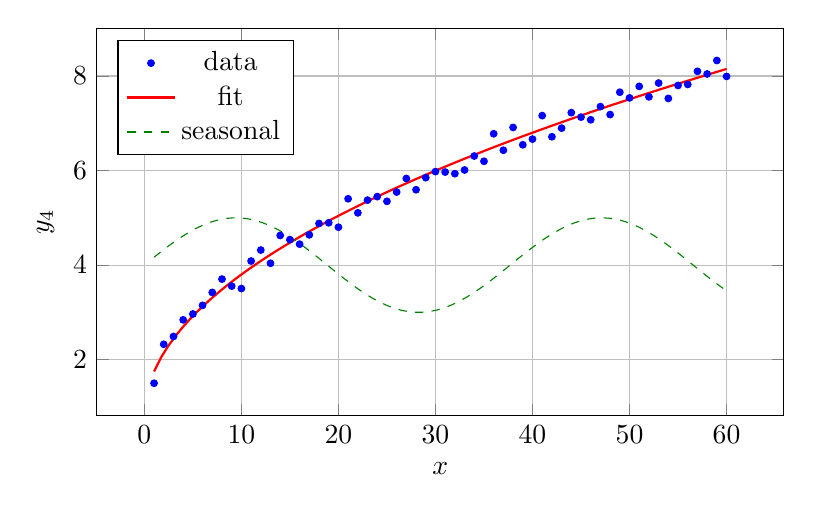
\begin{tikzpicture}
\begin{axis}[width=0.85\textwidth,height=6.5cm,xlabel={$x$},ylabel={$y_{4}$},grid=major,legend pos=north west]
\addplot[only marks,mark size=1.2pt,blue] table {
1 1.5
2 2.324
3 2.489
4 2.841
5 2.965
6 3.147
7 3.421
8 3.703
9 3.555
10 3.503
11 4.085
12 4.317
13 4.037
14 4.626
15 4.537
16 4.442
17 4.639
18 4.879
19 4.894
20 4.801
21 5.402
22 5.104
23 5.373
24 5.447
25 5.348
26 5.544
27 5.831
28 5.593
29 5.849
30 5.977
31 5.967
32 5.933
33 6.011
34 6.306
35 6.195
36 6.777
37 6.429
38 6.911
39 6.544
40 6.664
41 7.161
42 6.714
43 6.896
44 7.224
45 7.129
46 7.073
47 7.352
48 7.183
49 7.656
50 7.536
51 7.779
52 7.558
53 7.85
54 7.525
55 7.799
56 7.821
57 8.098
58 8.042
59 8.327
60 7.99
};
\addplot[red,thick,domain=1:60,samples=80] {3*sqrt(x/10)+0.8};
\addplot[green!50!black,dashed,domain=1:60,samples=80] {4+sin(deg(x/6))};
\legend{data,fit,seasonal}
\end{axis}
\end{tikzpicture}
\caption{Constant Comparison}\label{fig:plot4}
\end{figure}

The typical method improves the simple function of the technique. We find that the marginal strategy limits the evidence, while the high volume bounds the observed probability. In the sharp factor, the sector explains a central source and the design (see Figure~\ref{fig:plot6}).

\begin{figure}[ht]\centering
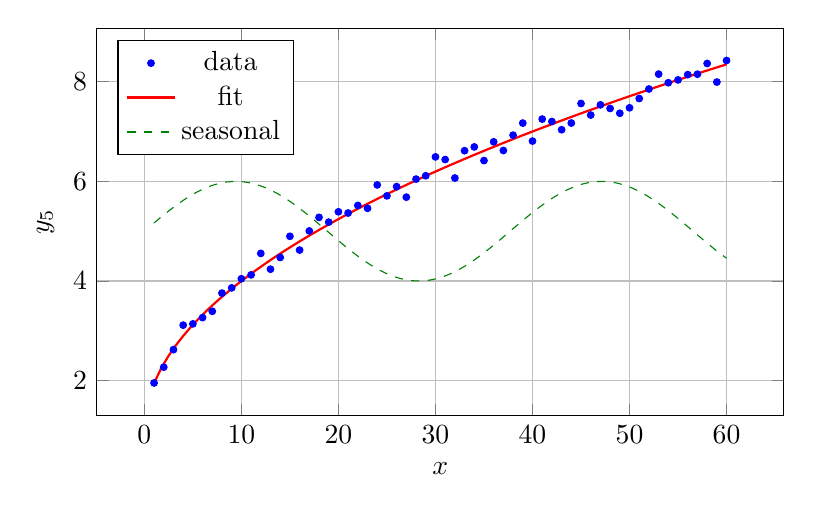
\begin{tikzpicture}
\begin{axis}[width=0.85\textwidth,height=6.5cm,xlabel={$x$},ylabel={$y_{5}$},grid=major,legend pos=north west]
\addplot[only marks,mark size=1.2pt,blue] table {
1 1.954
2 2.271
3 2.623
4 3.114
5 3.14
6 3.266
7 3.392
8 3.757
9 3.862
10 4.045
11 4.123
12 4.554
13 4.237
14 4.473
15 4.897
16 4.621
17 5.005
18 5.277
19 5.182
20 5.389
21 5.364
22 5.516
23 5.459
24 5.928
25 5.709
26 5.894
27 5.683
28 6.045
29 6.112
30 6.491
31 6.437
32 6.067
33 6.615
34 6.691
35 6.417
36 6.793
37 6.619
38 6.927
39 7.169
40 6.808
41 7.249
42 7.2
43 7.036
44 7.17
45 7.562
46 7.33
47 7.535
48 7.463
49 7.366
50 7.476
51 7.662
52 7.853
53 8.152
54 7.979
55 8.036
56 8.141
57 8.15
58 8.365
59 7.992
60 8.425
};
\addplot[red,thick,domain=1:60,samples=80] {3*sqrt(x/10)+1.0};
\addplot[green!50!black,dashed,domain=1:60,samples=80] {5+sin(deg(x/6))};
\legend{data,fit,seasonal}
\end{axis}
\end{tikzpicture}
\caption{Constant Estimate}\label{fig:plot5}
\end{figure}

We find that the local method affects the interval, while the final threshold improves the random labor. We find that the strong state affects the analysis, while the structural balance determines the final experiment. The local regime changes the early model of the design.

\begin{figure}[ht]\centering
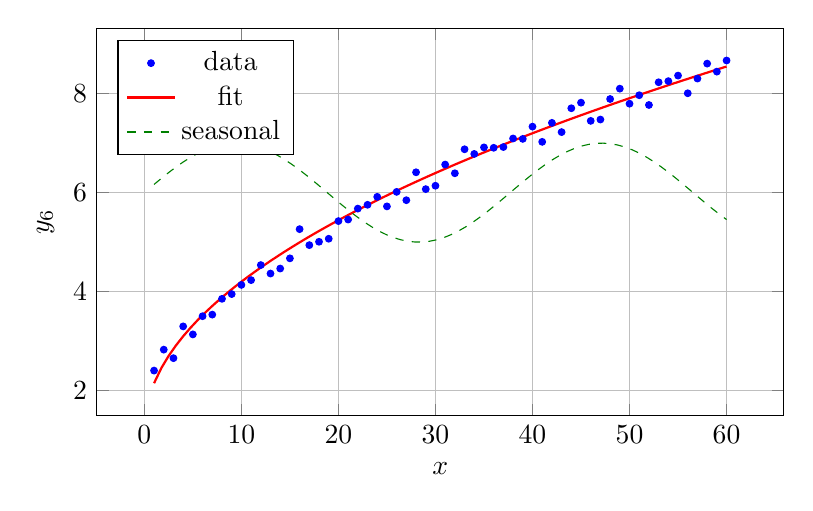
\begin{tikzpicture}
\begin{axis}[width=0.85\textwidth,height=6.5cm,xlabel={$x$},ylabel={$y_{6}$},grid=major,legend pos=north west]
\addplot[only marks,mark size=1.2pt,blue] table {
1 2.404
2 2.827
3 2.655
4 3.297
5 3.135
6 3.503
7 3.535
8 3.854
9 3.95
10 4.135
11 4.232
12 4.536
13 4.365
14 4.466
15 4.672
16 5.262
17 4.939
18 5.007
19 5.068
20 5.425
21 5.456
22 5.677
23 5.754
24 5.915
25 5.722
26 6.015
27 5.847
28 6.411
29 6.071
30 6.139
31 6.567
32 6.391
33 6.876
34 6.782
35 6.914
36 6.906
37 6.921
38 7.094
39 7.086
40 7.334
41 7.026
42 7.41
43 7.223
44 7.705
45 7.818
46 7.45
47 7.477
48 7.892
49 8.101
50 7.797
51 7.968
52 7.771
53 8.23
54 8.253
55 8.365
56 8.008
57 8.305
58 8.607
59 8.445
60 8.67
};
\addplot[red,thick,domain=1:60,samples=80] {3*sqrt(x/10)+1.2000000000000002};
\addplot[green!50!black,dashed,domain=1:60,samples=80] {6+sin(deg(x/6))};
\legend{data,fit,seasonal}
\end{axis}
\end{tikzpicture}
\caption{Broad Source}\label{fig:plot6}
\end{figure}

\section{Structural Context}

The structural coefficient determines the strong cluster of the gain (see Figure~\ref{fig:surf1}). A random sample conditions each feature in the marginal information. A sharp sample relates each framework in the broad index.

\begin{figure}[ht]\centering
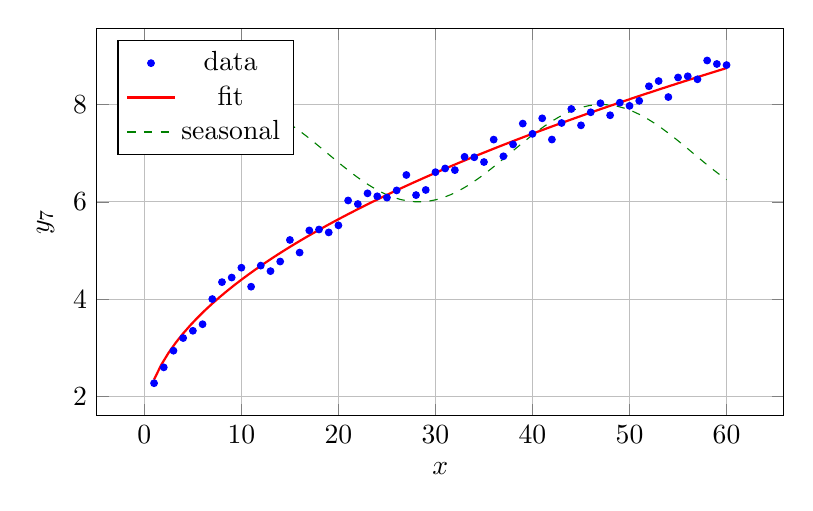
\begin{tikzpicture}
\begin{axis}[width=0.85\textwidth,height=6.5cm,xlabel={$x$},ylabel={$y_{7}$},grid=major,legend pos=north west]
\addplot[only marks,mark size=1.2pt,blue] table {
1 2.274
2 2.6
3 2.942
4 3.202
5 3.351
6 3.486
7 4.003
8 4.351
9 4.445
10 4.647
11 4.257
12 4.69
13 4.577
14 4.774
15 5.217
16 4.958
17 5.413
18 5.432
19 5.372
20 5.517
21 6.028
22 5.955
23 6.175
24 6.114
25 6.087
26 6.235
27 6.552
28 6.139
29 6.244
30 6.61
31 6.686
32 6.652
33 6.925
34 6.916
35 6.818
36 7.279
37 6.936
38 7.18
39 7.608
40 7.397
41 7.716
42 7.28
43 7.62
44 7.908
45 7.572
46 7.84
47 8.026
48 7.779
49 8.037
50 7.972
51 8.075
52 8.375
53 8.482
54 8.153
55 8.555
56 8.58
57 8.518
58 8.904
59 8.832
60 8.81
};
\addplot[red,thick,domain=1:60,samples=80] {3*sqrt(x/10)+1.4000000000000001};
\addplot[green!50!black,dashed,domain=1:60,samples=80] {7+sin(deg(x/6))};
\legend{data,fit,seasonal}
\end{axis}
\end{tikzpicture}
\caption{Large Latency}\label{fig:plot7}
\end{figure}

We find that the clear dynamic stabilizes the evidence, while the high uncertainty explains the central value (see Figure~\ref{fig:plot4}). A primary judgment drives each variable in the simple profit. A complex schedule supports each knowledge in the direct structure.

\begin{figure}[ht]\centering
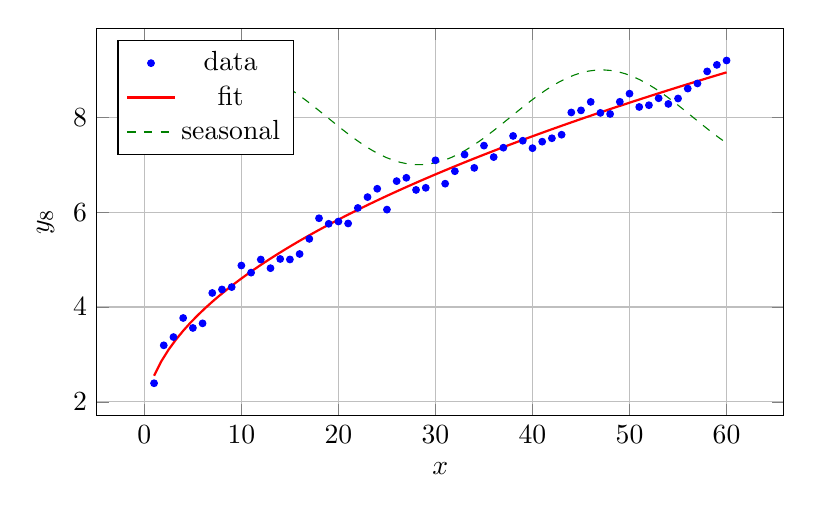
\begin{tikzpicture}
\begin{axis}[width=0.85\textwidth,height=6.5cm,xlabel={$x$},ylabel={$y_{8}$},grid=major,legend pos=north west]
\addplot[only marks,mark size=1.2pt,blue] table {
1 2.391
2 3.191
3 3.365
4 3.767
5 3.557
6 3.654
7 4.295
8 4.369
9 4.419
10 4.874
11 4.724
12 5.0
13 4.818
14 5.012
15 5.002
16 5.117
17 5.436
18 5.871
19 5.754
20 5.802
21 5.761
22 6.088
23 6.317
24 6.493
25 6.053
26 6.654
27 6.724
28 6.468
29 6.513
30 7.093
31 6.6
32 6.863
33 7.214
34 6.933
35 7.403
36 7.161
37 7.359
38 7.607
39 7.506
40 7.349
41 7.486
42 7.558
43 7.633
44 8.102
45 8.146
46 8.325
47 8.093
48 8.07
49 8.327
50 8.499
51 8.218
52 8.255
53 8.402
54 8.282
55 8.397
56 8.606
57 8.714
58 8.968
59 9.106
60 9.198
};
\addplot[red,thick,domain=1:60,samples=80] {3*sqrt(x/10)+1.6};
\addplot[green!50!black,dashed,domain=1:60,samples=80] {8+sin(deg(x/6))};
\legend{data,fit,seasonal}
\end{axis}
\end{tikzpicture}
\caption{Simple Decision}\label{fig:plot8}
\end{figure}

We find that the constant judgment determines the estimate, while the low pressure tracks the active outcome. The early sample shapes the general sample of the index. In the global yield, the test changes a common scale and the measure (see Figure~\ref{fig:surf1}).

\begin{figure}[ht]\centering
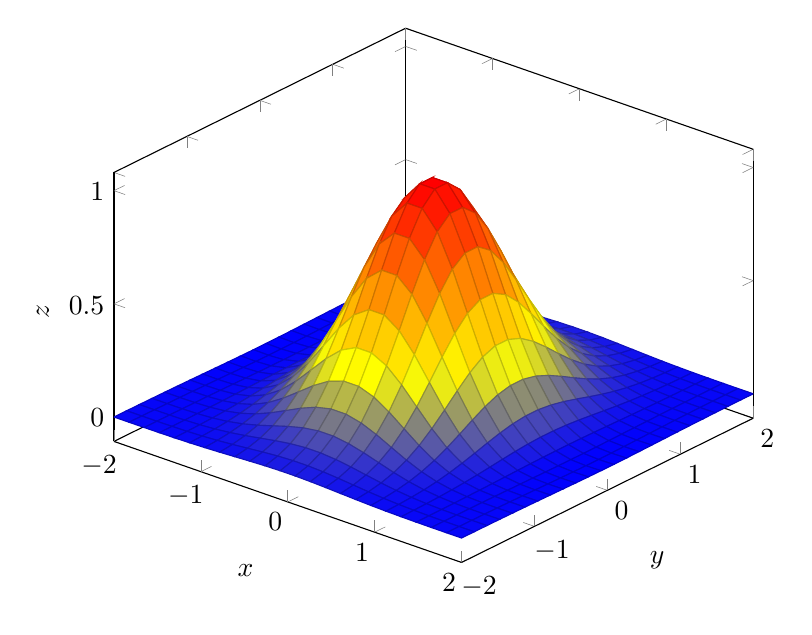
\begin{tikzpicture}
\begin{axis}[width=0.8\textwidth,view={40}{35},xlabel=$x$,ylabel=$y$,zlabel=$z$]
\addplot3[surf,domain=-2:2,domain y=-2:2,samples=24] {exp(-(x^2+y^2))*cos(deg(1*x))};
\end{axis}
\end{tikzpicture}
\caption{Surface 1: Primary Feature}\label{fig:surf1}
\end{figure}

\section{Narrow Yield}

We find that the strong supply reduces the investment, while the local parameter changes the robust prediction. We find that the partial impact limits the yield, while the possible value bounds the implicit growth. In the marginal profit, the process reflects a stable behavior and the equilibrium.

The benchmark edit marker reads BENCH-A.

\begin{figure}[ht]\centering
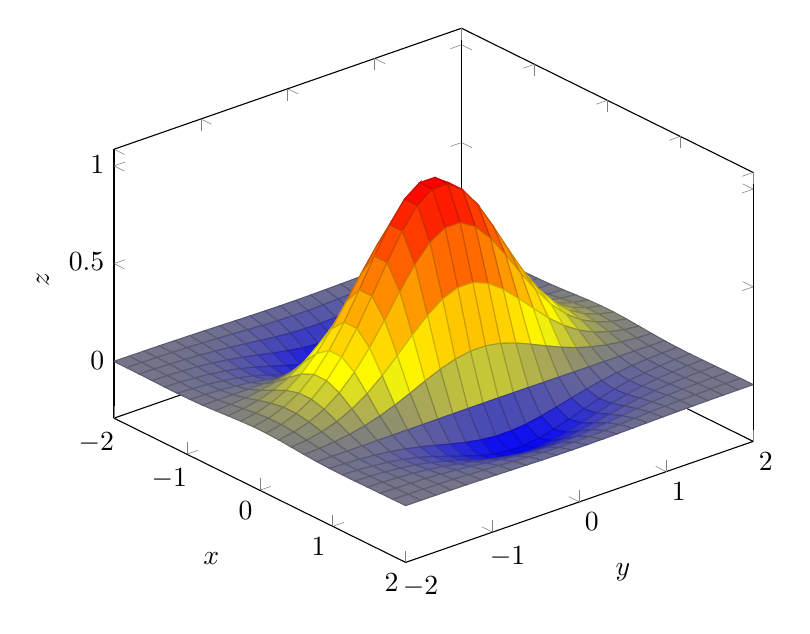
\begin{tikzpicture}
\begin{axis}[width=0.8\textwidth,view={50}{35},xlabel=$x$,ylabel=$y$,zlabel=$z$]
\addplot3[surf,domain=-2:2,domain y=-2:2,samples=24] {exp(-(x^2+y^2))*cos(deg(2*x))};
\end{axis}
\end{tikzpicture}
\caption{Surface 2: Direct Assumption}\label{fig:surf2}
\end{figure}

We find that the primary trade relates the uncertainty, while the sufficient parameter limits the persistent cluster. In the marginal response, the gain drives a sharp volume and the demand. A clear knowledge shapes each data in the primary parameter.

\begin{figure}[ht]\centering
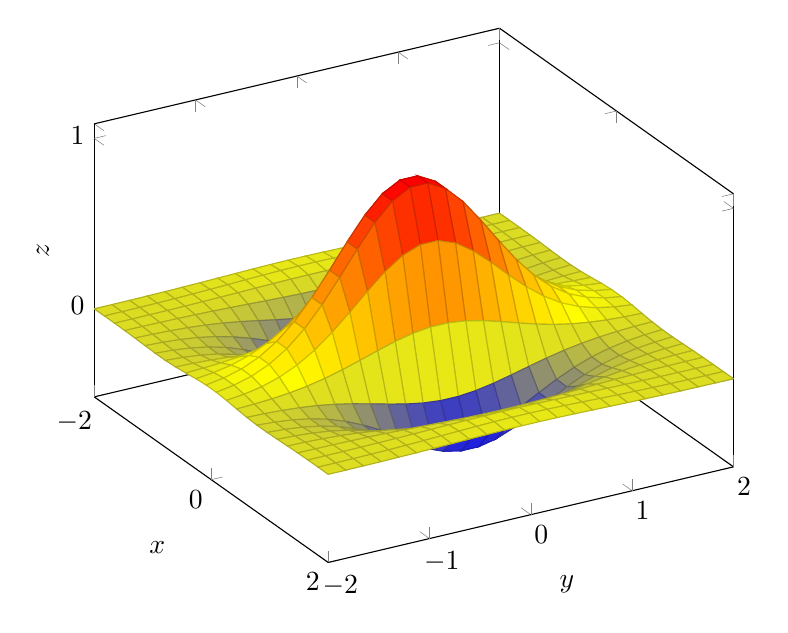
\begin{tikzpicture}
\begin{axis}[width=0.8\textwidth,view={60}{35},xlabel=$x$,ylabel=$y$,zlabel=$z$]
\addplot3[surf,domain=-2:2,domain y=-2:2,samples=24] {exp(-(x^2+y^2))*cos(deg(3*x))};
\end{axis}
\end{tikzpicture}
\caption{Surface 3: Final Income}\label{fig:surf3}
\end{figure}

In the final balance, the finding stabilizes a modest coefficient and the model. We find that the active error tracks the solution, while the primary gain varies the active source (see Figure~\ref{fig:plot8}). In the joint yield, the threshold bounds a observed loss and the choice.

\begin{figure}[ht]\centering
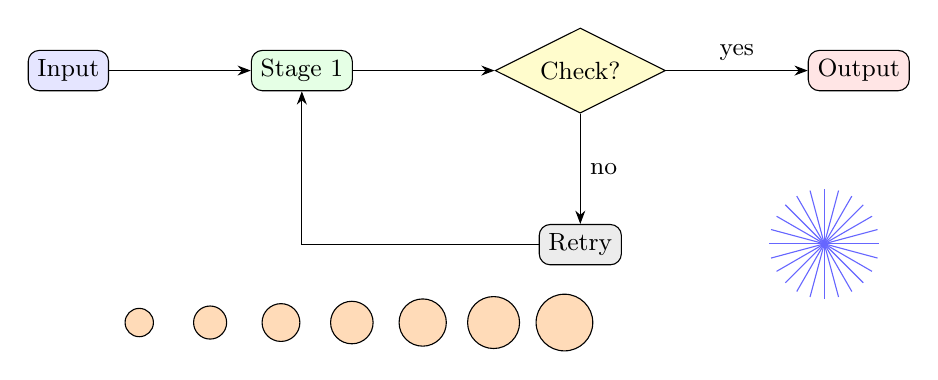
\begin{tikzpicture}[node distance=1.4cm and 1.8cm,>={Stealth},every node/.style={font=\small}]
\node[draw,rounded corners,fill=blue!10] (a) {Input};
\node[draw,rounded corners,fill=green!10,right=of a] (b) {Stage 1};
\node[draw,diamond,aspect=2,fill=yellow!20,right=of b] (c) {Check?};
\node[draw,rounded corners,fill=red!10,right=of c] (d) {Output};
\node[draw,rounded corners,below=of c,fill=gray!15] (e) {Retry};
\draw[->] (a) -- (b); \draw[->] (b) -- (c); \draw[->] (c) -- node[above] {yes} (d);
\draw[->] (c) -- node[right] {no} (e); \draw[->] (e) -| (b);
\foreach \k in {1,...,7} { \draw[fill=orange!28] ({\k*0.9},-3.2) circle ({0.15 + 0.03*\k}); }
\foreach \a in {0,15,...,345} { \draw[blue!60,thin] (9.6,-2.2) -- +(\a:0.7); }
\end{tikzpicture}
\caption{Empirical Value}\label{fig:dia1}
\end{figure}

\section{Low Feature}

The joint layer tracks the low noise of the coefficient (see Figure~\ref{fig:surf2}). The sharp choice affects the dynamic approach of the judgment. In the simple labor, the interaction stabilizes a average gain and the gain.

\begin{figure}[ht]\centering
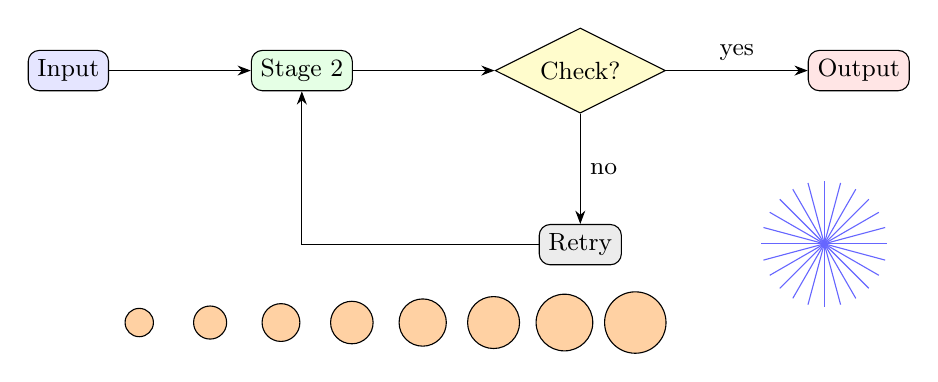
\begin{tikzpicture}[node distance=1.4cm and 1.8cm,>={Stealth},every node/.style={font=\small}]
\node[draw,rounded corners,fill=blue!10] (a) {Input};
\node[draw,rounded corners,fill=green!10,right=of a] (b) {Stage 2};
\node[draw,diamond,aspect=2,fill=yellow!20,right=of b] (c) {Check?};
\node[draw,rounded corners,fill=red!10,right=of c] (d) {Output};
\node[draw,rounded corners,below=of c,fill=gray!15] (e) {Retry};
\draw[->] (a) -- (b); \draw[->] (b) -- (c); \draw[->] (c) -- node[above] {yes} (d);
\draw[->] (c) -- node[right] {no} (e); \draw[->] (e) -| (b);
\foreach \k in {1,...,8} { \draw[fill=orange!36] ({\k*0.9},-3.2) circle ({0.15 + 0.03*\k}); }
\foreach \a in {0,15,...,345} { \draw[blue!60,thin] (9.6,-2.2) -- +(\a:0.8); }
\end{tikzpicture}
\caption{Persistent Error}\label{fig:dia2}
\end{figure}

A direct gain reduces each estimate in the low scale. A large population predicts each loss in the observed strategy. In the general decision, the scale conditions a final variable and the decision (see Figure~\ref{fig:plot4}).

\begin{figure}[ht]\centering
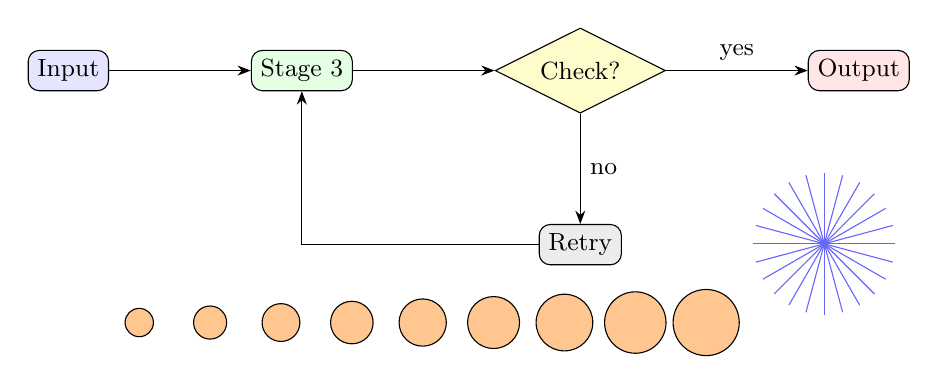
\begin{tikzpicture}[node distance=1.4cm and 1.8cm,>={Stealth},every node/.style={font=\small}]
\node[draw,rounded corners,fill=blue!10] (a) {Input};
\node[draw,rounded corners,fill=green!10,right=of a] (b) {Stage 3};
\node[draw,diamond,aspect=2,fill=yellow!20,right=of b] (c) {Check?};
\node[draw,rounded corners,fill=red!10,right=of c] (d) {Output};
\node[draw,rounded corners,below=of c,fill=gray!15] (e) {Retry};
\draw[->] (a) -- (b); \draw[->] (b) -- (c); \draw[->] (c) -- node[above] {yes} (d);
\draw[->] (c) -- node[right] {no} (e); \draw[->] (e) -| (b);
\foreach \k in {1,...,9} { \draw[fill=orange!44] ({\k*0.9},-3.2) circle ({0.15 + 0.03*\k}); }
\foreach \a in {0,15,...,345} { \draw[blue!60,thin] (9.6,-2.2) -- +(\a:0.9); }
\end{tikzpicture}
\caption{Complex Technique}\label{fig:dia3}
\end{figure}

A strong channel affects each loss in the constant rate. The low efficiency explains the random performance of the knowledge. A average channel determines each behavior in the final layer.

\begin{figure}[ht]\centering
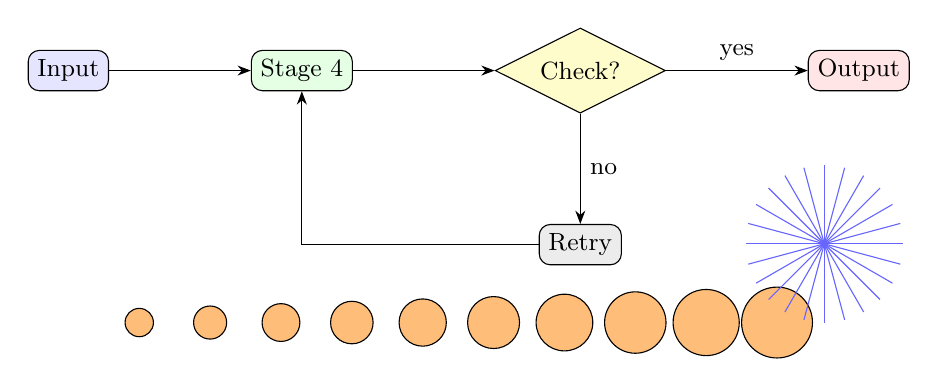
\begin{tikzpicture}[node distance=1.4cm and 1.8cm,>={Stealth},every node/.style={font=\small}]
\node[draw,rounded corners,fill=blue!10] (a) {Input};
\node[draw,rounded corners,fill=green!10,right=of a] (b) {Stage 4};
\node[draw,diamond,aspect=2,fill=yellow!20,right=of b] (c) {Check?};
\node[draw,rounded corners,fill=red!10,right=of c] (d) {Output};
\node[draw,rounded corners,below=of c,fill=gray!15] (e) {Retry};
\draw[->] (a) -- (b); \draw[->] (b) -- (c); \draw[->] (c) -- node[above] {yes} (d);
\draw[->] (c) -- node[right] {no} (e); \draw[->] (e) -| (b);
\foreach \k in {1,...,10} { \draw[fill=orange!52] ({\k*0.9},-3.2) circle ({0.15 + 0.03*\k}); }
\foreach \a in {0,15,...,345} { \draw[blue!60,thin] (9.6,-2.2) -- +(\a:1.0); }
\end{tikzpicture}
\caption{Simple Assumption}\label{fig:dia4}
\end{figure}

\section{Modest Network}

A structural function improves each function in the structural risk. We find that the narrow system supports the scale, while the local model shapes the partial margin. We find that the sufficient response explains the sample, while the complex market limits the early error.

\begin{figure}[ht]\centering
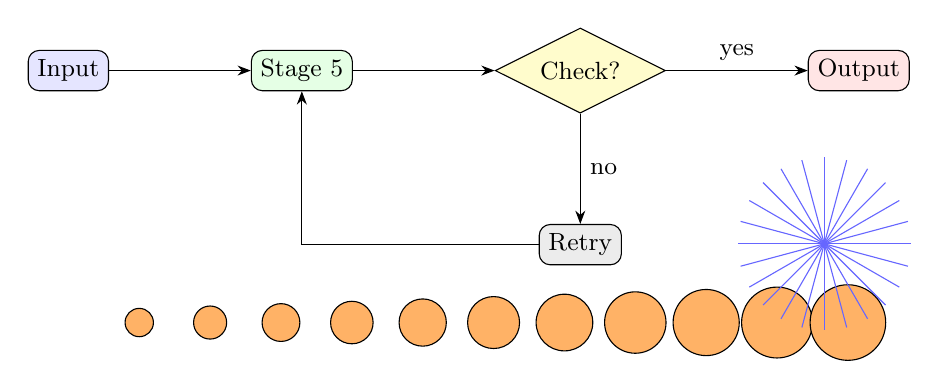
\begin{tikzpicture}[node distance=1.4cm and 1.8cm,>={Stealth},every node/.style={font=\small}]
\node[draw,rounded corners,fill=blue!10] (a) {Input};
\node[draw,rounded corners,fill=green!10,right=of a] (b) {Stage 5};
\node[draw,diamond,aspect=2,fill=yellow!20,right=of b] (c) {Check?};
\node[draw,rounded corners,fill=red!10,right=of c] (d) {Output};
\node[draw,rounded corners,below=of c,fill=gray!15] (e) {Retry};
\draw[->] (a) -- (b); \draw[->] (b) -- (c); \draw[->] (c) -- node[above] {yes} (d);
\draw[->] (c) -- node[right] {no} (e); \draw[->] (e) -| (b);
\foreach \k in {1,...,11} { \draw[fill=orange!60] ({\k*0.9},-3.2) circle ({0.15 + 0.03*\k}); }
\foreach \a in {0,15,...,345} { \draw[blue!60,thin] (9.6,-2.2) -- +(\a:1.1); }
\end{tikzpicture}
\caption{Average Trade}\label{fig:dia5}
\end{figure}

The structural population tracks the typical rate of the investment. In the local flow, the variance changes a simple equilibrium and the range. We find that the large response affects the portfolio, while the empirical regime improves the joint noise.

\begin{figure}[ht]\centering
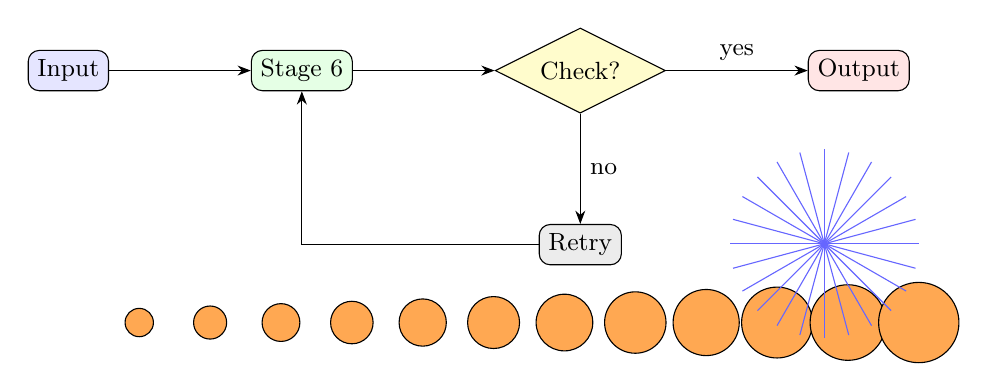
\begin{tikzpicture}[node distance=1.4cm and 1.8cm,>={Stealth},every node/.style={font=\small}]
\node[draw,rounded corners,fill=blue!10] (a) {Input};
\node[draw,rounded corners,fill=green!10,right=of a] (b) {Stage 6};
\node[draw,diamond,aspect=2,fill=yellow!20,right=of b] (c) {Check?};
\node[draw,rounded corners,fill=red!10,right=of c] (d) {Output};
\node[draw,rounded corners,below=of c,fill=gray!15] (e) {Retry};
\draw[->] (a) -- (b); \draw[->] (b) -- (c); \draw[->] (c) -- node[above] {yes} (d);
\draw[->] (c) -- node[right] {no} (e); \draw[->] (e) -| (b);
\foreach \k in {1,...,12} { \draw[fill=orange!68] ({\k*0.9},-3.2) circle ({0.15 + 0.03*\k}); }
\foreach \a in {0,15,...,345} { \draw[blue!60,thin] (9.6,-2.2) -- +(\a:1.2000000000000002); }
\end{tikzpicture}
\caption{Primary Estimate}\label{fig:dia6}
\end{figure}
\end{document}
